\mysubsectionformatted{SOSE - Service Oriented Software Engineering}
\myparagraph{
    Le parole chiave che determinano questo approccio sono la riusabilità e l'uso di servizi software (per il CBSE era l'uso
    dei componenti software).
    \\
    Questo approccio nasce con lo scopo di fornire lo stesso servizio a più applicazioni o utenti, questo perché i servizi
    sono indipendenti tra loro.
    \\
    Per servizio si intende un'entità software con basso accoppiamento (loosely-coupled) che incapsula delle funzionalità che
    possono essere distribuite e accesse.

    \mysubsubsectionformatted{Standard di SOSE}
    \begin{center}
        \begin{tabularx}{\textwidth}{|>{\centering}m{2cm}|X|}
            \hline
            \textbf{SOAP} & Protocollo di accesso agli oggetti che definisce un'organizzazione per lo scambio di dati strutturati tra i web services.                                          \\ \hline
            \textbf{WSDL} & Definisce come possono essere rappresentate le interfacce dei web services.                                                                                        \\ \hline
            \textbf{UDDI} & Standard di ricerca che definisce come possono essere organizzate le informazioni di descrizione dei servizi, utilizzate dai richiedenti dei servizi per trovarli. \\ \hline
        \end{tabularx}
    \end{center}

    \subsubsection{Illustrazione dell'approccio SOSE}
    \begin{center}
        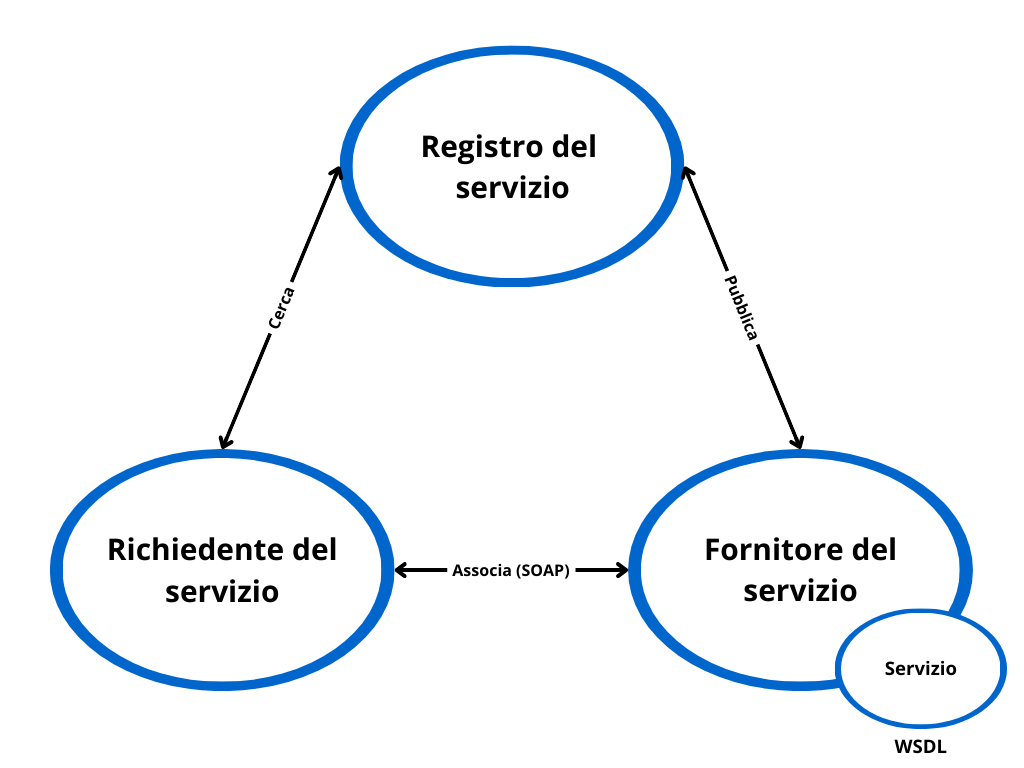
\includegraphics[width=10cm]{sose/funzionamento_sose.png}
    \end{center}
    \newpage

    \noindent Come per CBSE, anche SOSE distingue, nel suo caso, i servizi PER il riuso e i servizi CON riuso:
    \mysubsubsectionformatted{Servizi per il riuso}
    Come dice il titolo, questi servizi vengono sviluppati con lo scopo di essere riutilizzati all'interno di applicazioni orientati
    ai servizi. Questi servizi devono essere progettati come delle 'astrazioni riutilizzabili' che possono essere usati in sistemi diversi,
    in modo da poter garantire un servizio robusto e affidabile. Alla fine, il servizio deve essere ben documentato
    in modo da poter essere scoperto e capito da potenziali utenti.

    \mysubsubsectionformatted{Servizi con riuso}
    I servizi in questo caso vengono visti come dei componenti riutilizzabili. In questo modo, i servizi possono essere forniti localmente o
    esternamente verso altri fornitori. Altro vantaggio è che i servizi sono indipendenti dal linguaggio in cui vengono scritti, e per concludere
    l'investimento fatto in sistemi informatici obsoleti può essere preservato, conservandone quindi il valore attraverso aggiornamenti o
    modernizzazioni.

    \mysubsubsectionformatted{CBSE vs SOSE}
    La differenza sostanziale tra i due è che CBSE fa uso dei componenti, SOSE dei servizi.
    \begin{enumerate}
        \item I servizi sono indipendenti, i componenti no.
        \item I servizi non possiedono alcuna interfaccia 'richiesta'.
        \item La comunicazione tra i servizi avviene tramite messaggi in formato XML.
    \end{enumerate}
    \newpage
}